\subsection{Learning correspondence}
\begin{frame}[allowframebreaks]{Learning correspondence}
    \textbf{Training data:} Video frames, corresponding optical flow maps \\[1em]

    \textbf{Pretext task:} Predict the optical flow between pairs of video frames. \\[1em]
    \textbf{Learning Correspondence:}

    \begin{itemize}
        \item Match patches across frames
        \item Applications: tracking, correspondence learning
    \end{itemize}
\framebreak
    \textbf{Ultimate Goal:} Correspondence
    \begin{figure}
        \centering
        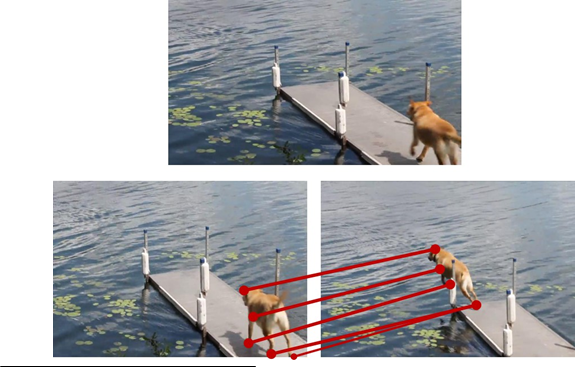
\includegraphics[width=1\textwidth,height=0.7\textheight,keepaspectratio]{images/video/slide_47_1_img.png}
    \end{figure}
    \footnotesize{[Wang and Efros, Learning Correspondence from the Cycle-consistency of Time, CVPR 2019]}
\end{frame}